\documentclass[12pt,letterpaper]{article}
\usepackage[utf8]{inputenc}
\usepackage{amsmath}
\usepackage{amsfonts}
\usepackage{amssymb}
\usepackage{amsthm}
\usepackage{graphicx}

\usepackage{hyperref}
\hypersetup{
    colorlinks=true,
    linkcolor=blue,
    filecolor=magenta,      
    urlcolor=cyan,
}
\urlstyle{same}

\usepackage{tabularx}
\usepackage[left=2cm,right=2cm,top=2cm,bottom=2cm]{geometry}
\usepackage{fancyhdr}
\usepackage{multicol}
\usepackage{multirow,array}
\usepackage{newtxtext,newtxmath}
\usepackage{relsize}
\usepackage{lastpage}
\usepackage{enumitem}
\usepackage{adjustbox}
\newcolumntype{Y}{>{\centering\arraybackslash}X}
	\setenumerate[1]{label={\bf Q\theenumi: ~}}
	\setenumerate[2]{label={\bf \theenumii: ~}}
\pagestyle{fancy}
\fancyhf{}
\lhead{BHCC Mat-181}
\rhead{\textsc{Standard normal probability problems}}
\rfoot{Page \thepage ~of \pageref*{LastPage}}



\begin{document}

%\newcommand{\emptybox}{\fbox{\phantom{\cfrac{aafkfhhhhha}{s}}}}
\newcommand{\emptybox}{\fbox{\text{ }\hspace{60pt}\text{ \phantom{$\cfrac{h}{h}$} }}}
\begin{enumerate}
\item For each of the following, complete the diagram so it has a shaded region and a probability statement, like in the example below.
\\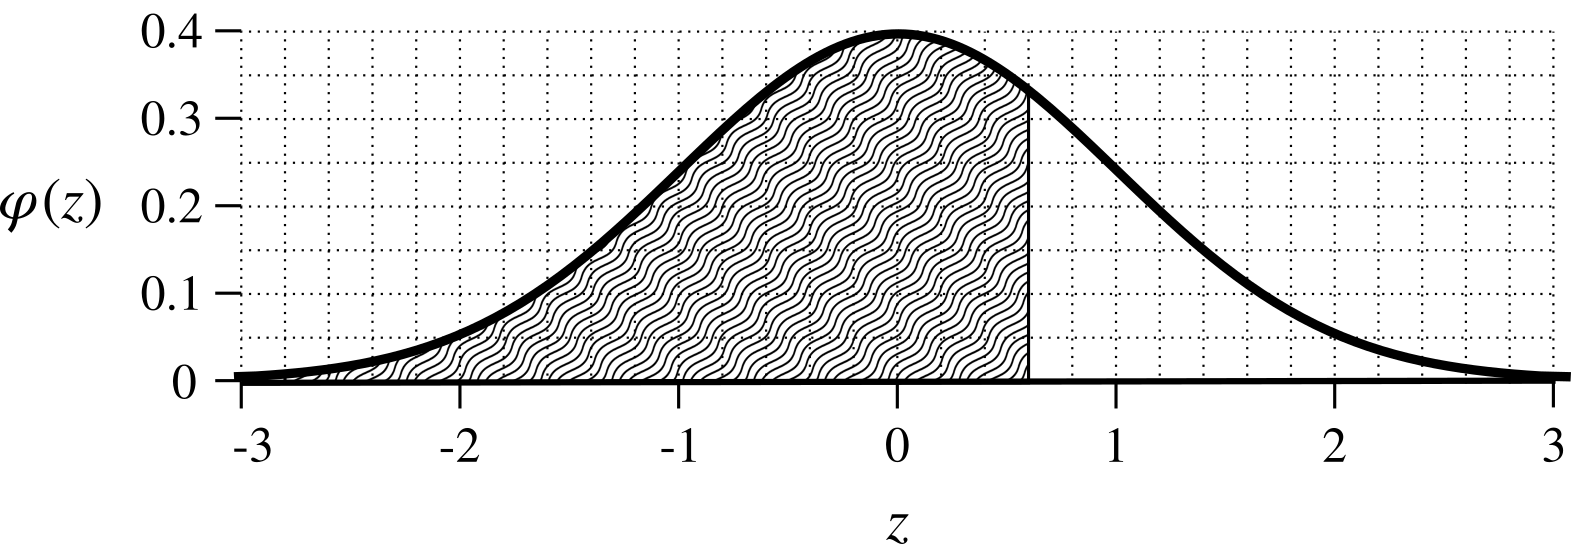
\includegraphics[scale=0.7]{0p6.png} $P(Z<0.6) = 0.7257$
\begin{enumerate}
\vfill
\item Shade the region and evaluate the probability $P(Z<-1.4)$.
\\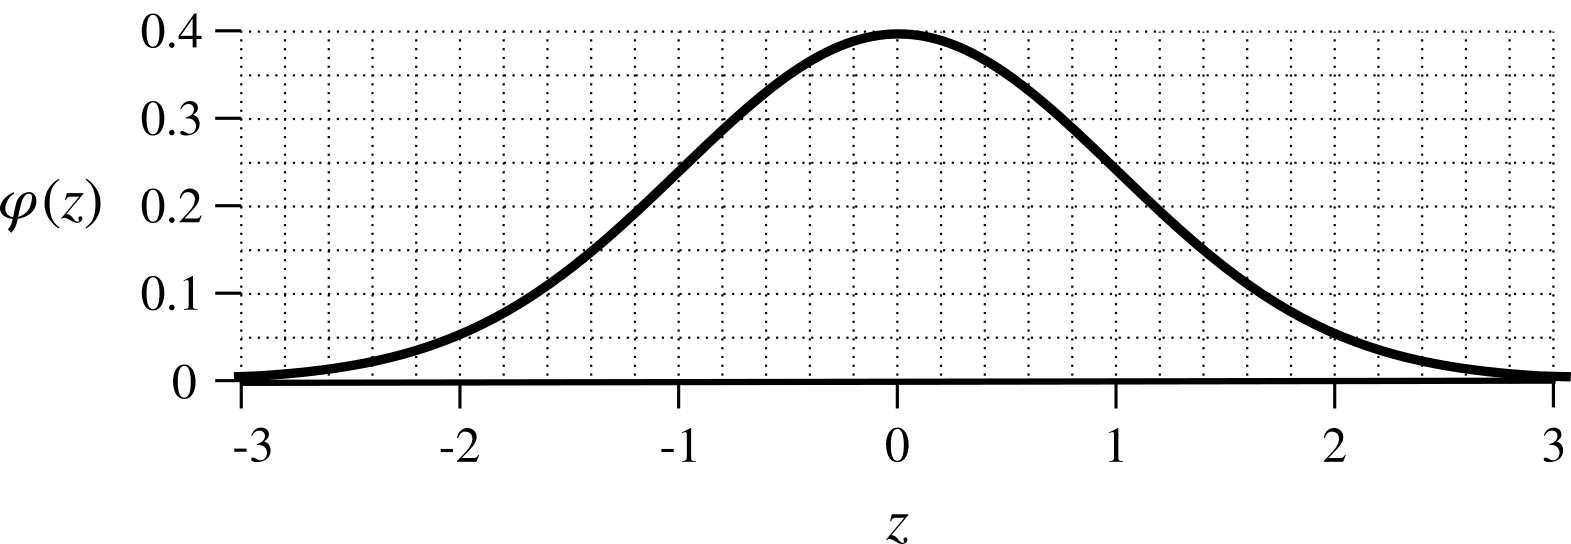
\includegraphics[scale=0.7]{blank.png} $P(Z<-1.4)=\emptybox$
\vfill
\item Shade the region and evaluate the probability $P(Z<2)$.
\\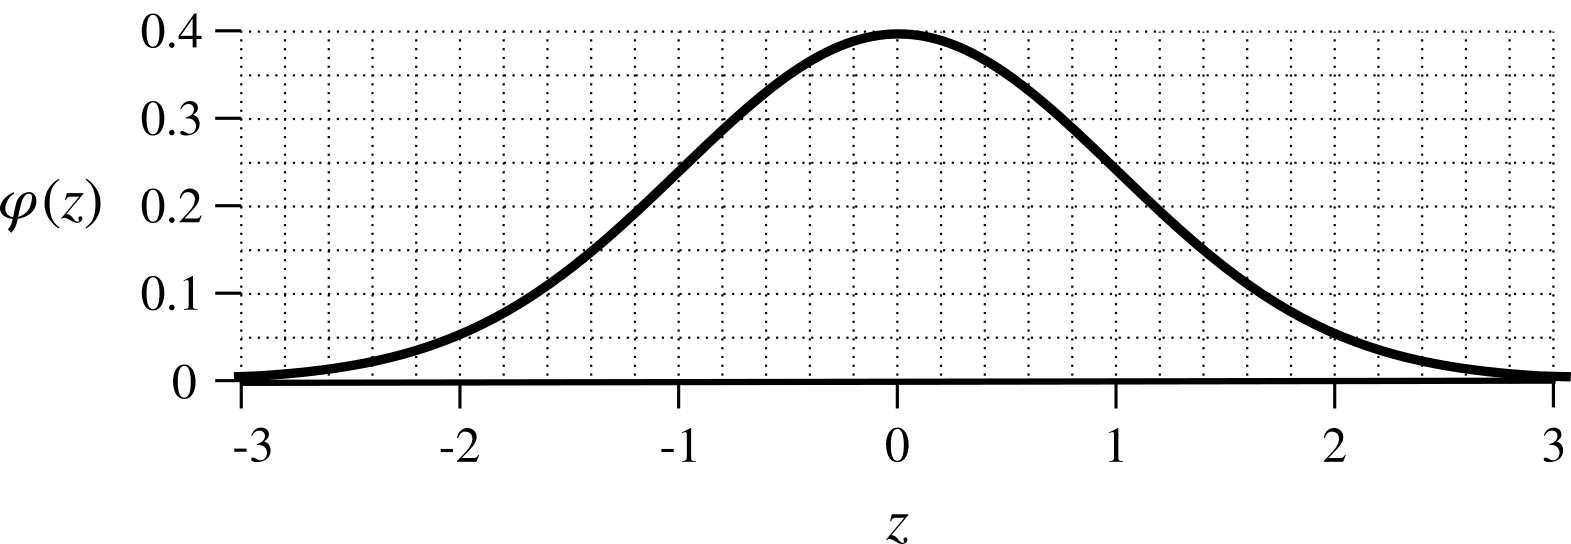
\includegraphics[scale=0.7]{blank.png} $P(Z<2)=\emptybox$
\vfill
\item From the shaded region, evaluate the probability.
\\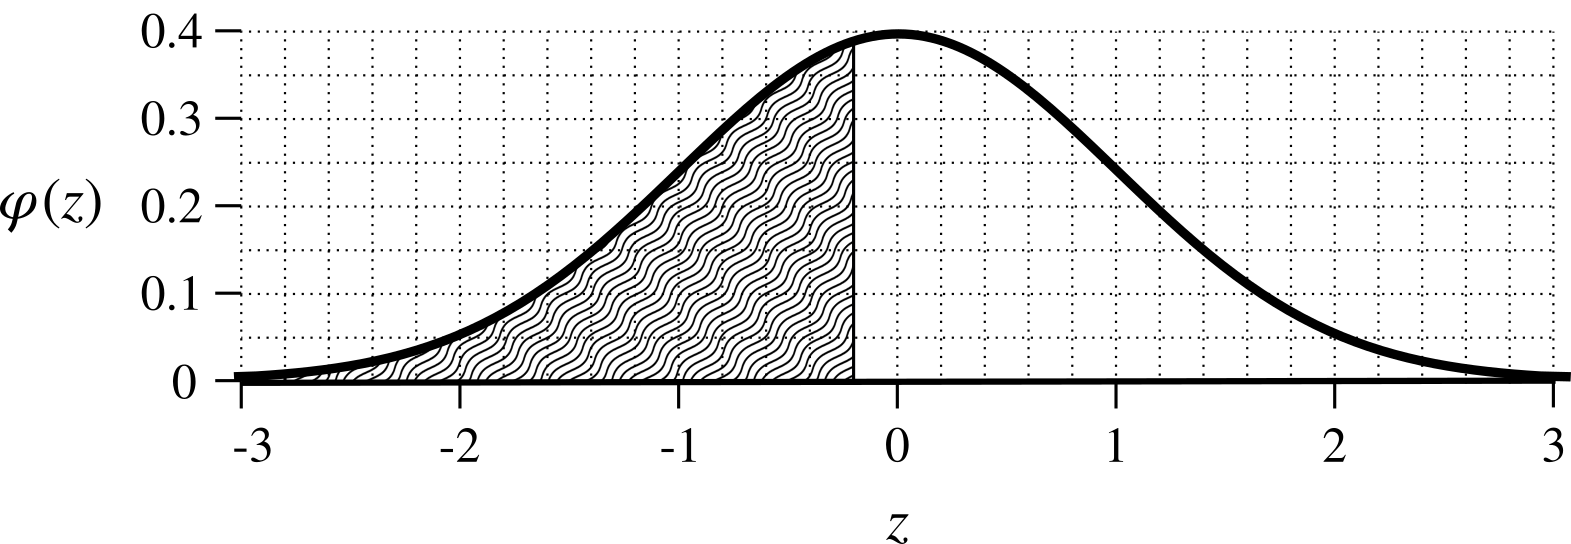
\includegraphics[scale=0.7]{n0p2.png}  $\emptybox=\emptybox$
\vfill
\end{enumerate}
\end{enumerate}

\newpage
The area under $\varphi(z)$ from $-\infty$ to $\infty$ is 1. Also, the function $\varphi(z)$ is symmetric. This leads to a useful property:
$$\Phi(-z) = 1-\Phi(z) $$
\begin{center}
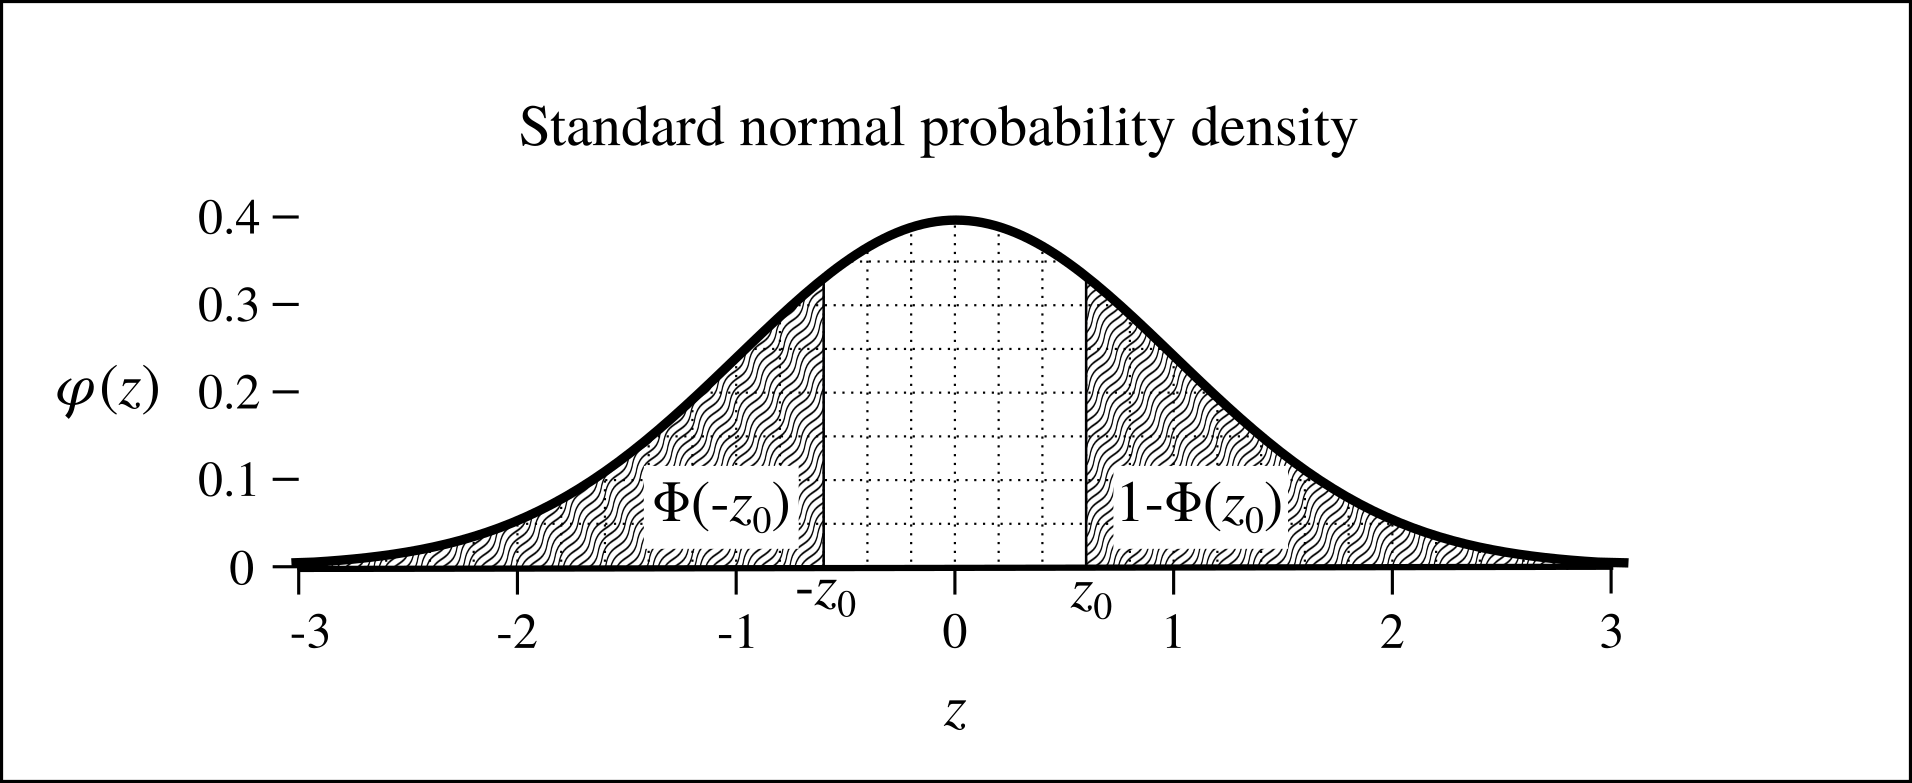
\includegraphics[scale=0.7]{prop.png}
\end{center}

There are five common areas we are asked to find: left, right, sectional, central (symmetric), and two-tailed (symmetric).
\begin{center}
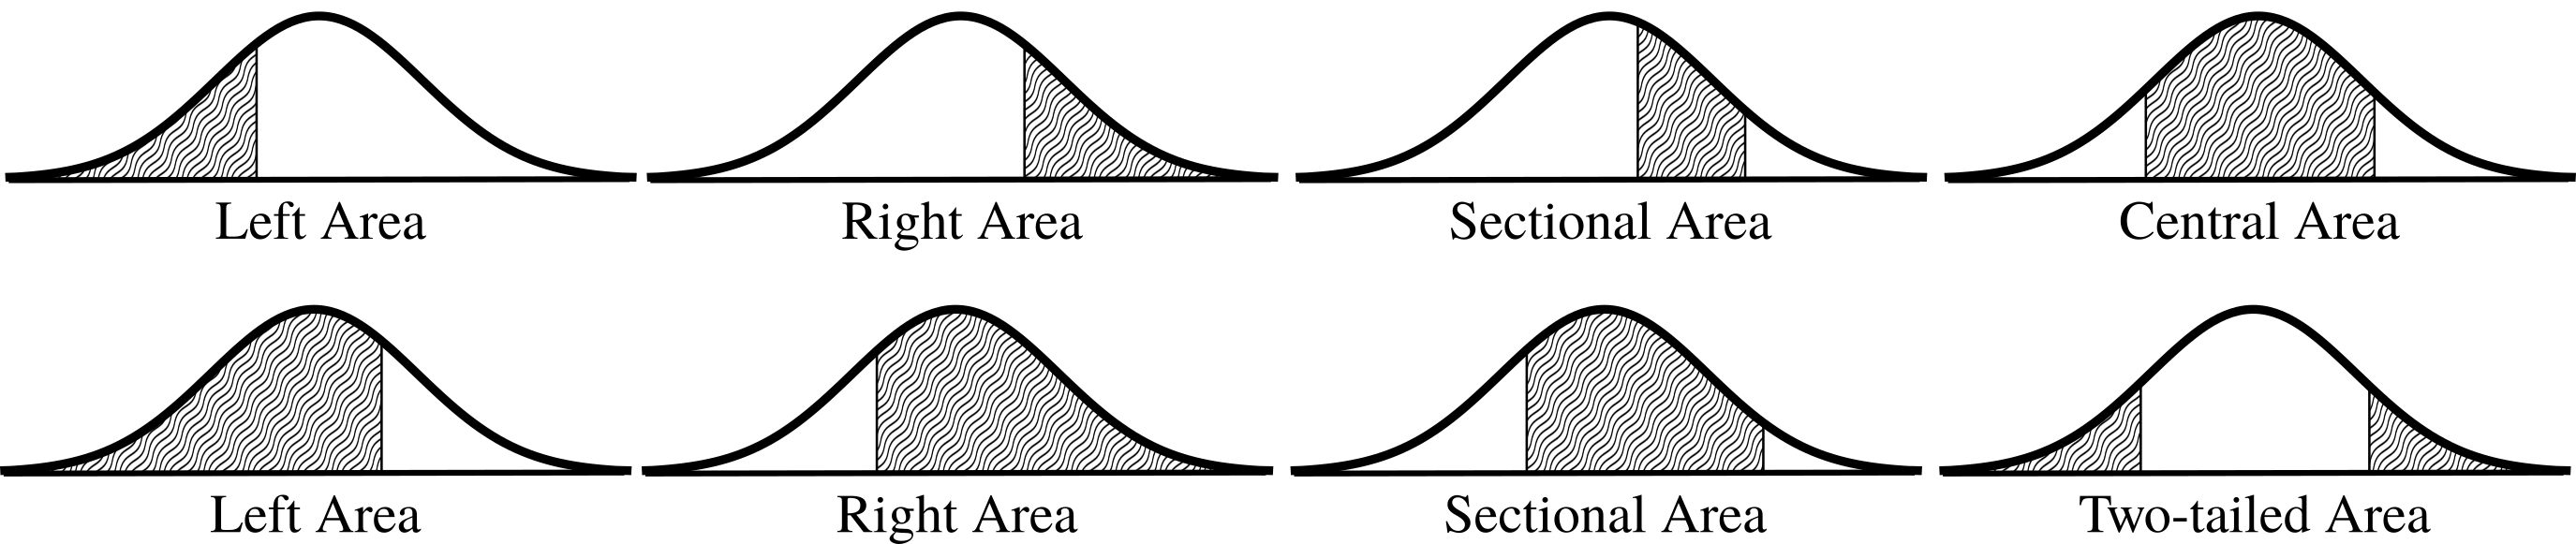
\includegraphics[scale=0.7]{types.png}
\end{center}
\begin{align*}
\texttt{Left area} &= P(Z<z)\\
 &= \Phi(z)\\\\
\texttt{Right area} &= P(Z>z) \\&= 1-\Phi(z) \\&= \Phi(-z)\\\\
\texttt{Sectional area} &= P(z_1<Z<z_2) \\&= \Phi(z_2) - \Phi(z_1)\\\\
\texttt{Central area} &= P(|Z|<z) \\&= \Phi(z)-\Phi(-z) \\&= 1-2\Phi(-z)\\ &= 2\Phi(z)-1\\\\
\texttt{Two-tailed area} &= P(|Z|>z) \\ &= 1-\Phi(z)+\Phi(-z) \\&=2-2\Phi(z) \\ &= 2\Phi(-z)
\end{align*}
\label{hi}

\newpage
\begin{enumerate}[resume]
\item For each of the following, complete the diagram so it has a shaded region and a probability statement. Also, notice that you can estimate the probability by counting the number of shaded squares; each unit square is worth 1\%.
\begin{enumerate}
\item Shade the region of and evaluate the probability that $Z$ is more than 1.6.
\\ 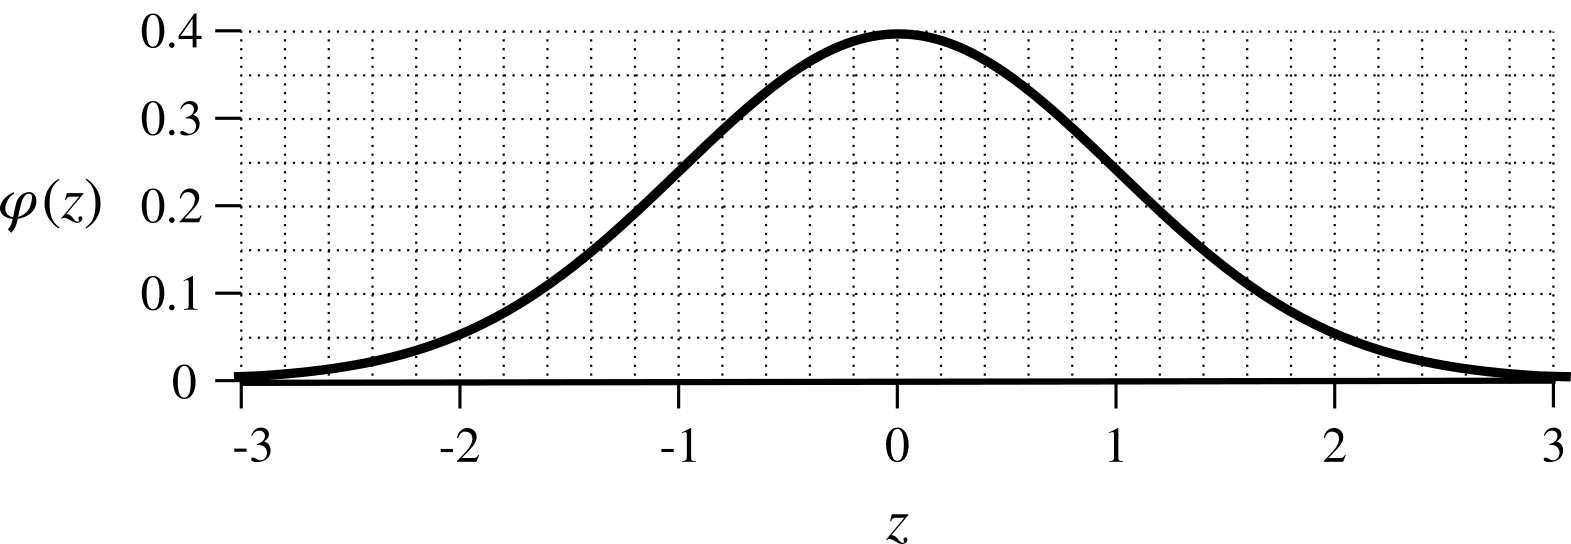
\includegraphics[scale=0.7]{blank.png}   $~~\emptybox=\emptybox$
\vfill
\item Shade the region of and evaluate the probability that $Z$ is between 0.4 and 0.6.
\\ 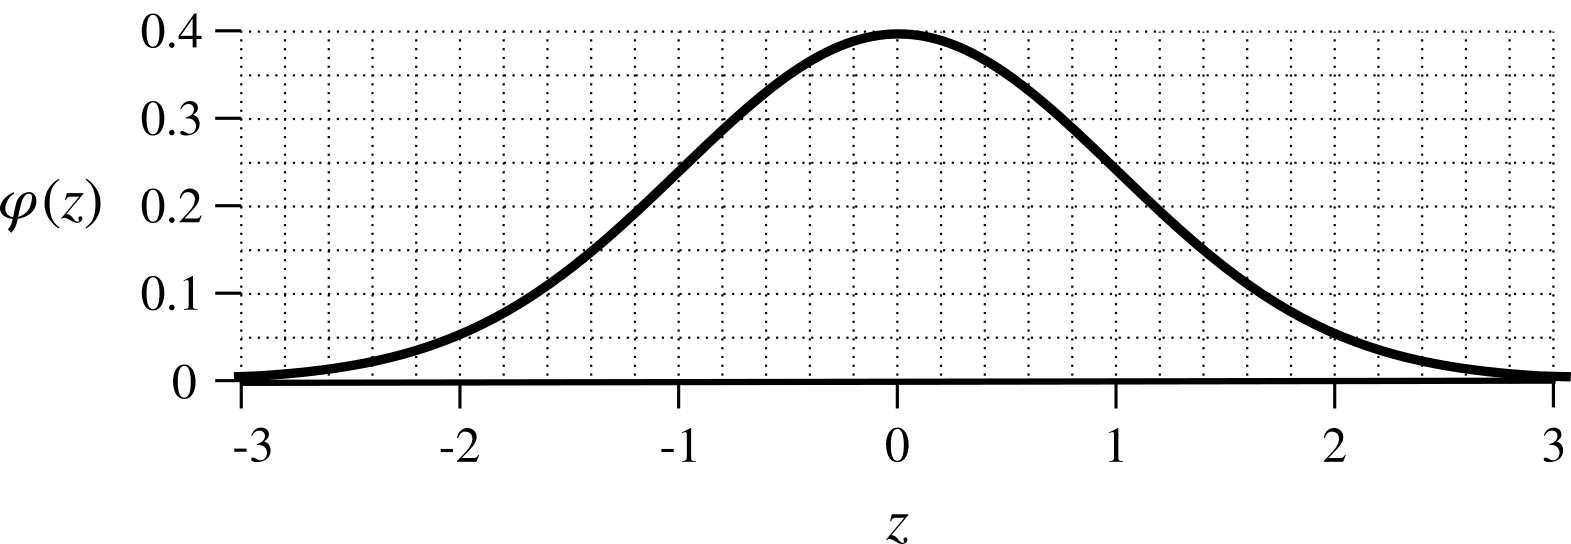
\includegraphics[scale=0.7]{blank.png}   $~~\emptybox=\emptybox$
\vfill
\item Shade the region of and evaluate the probability that $Z$ is between 1 and 2.
\\ 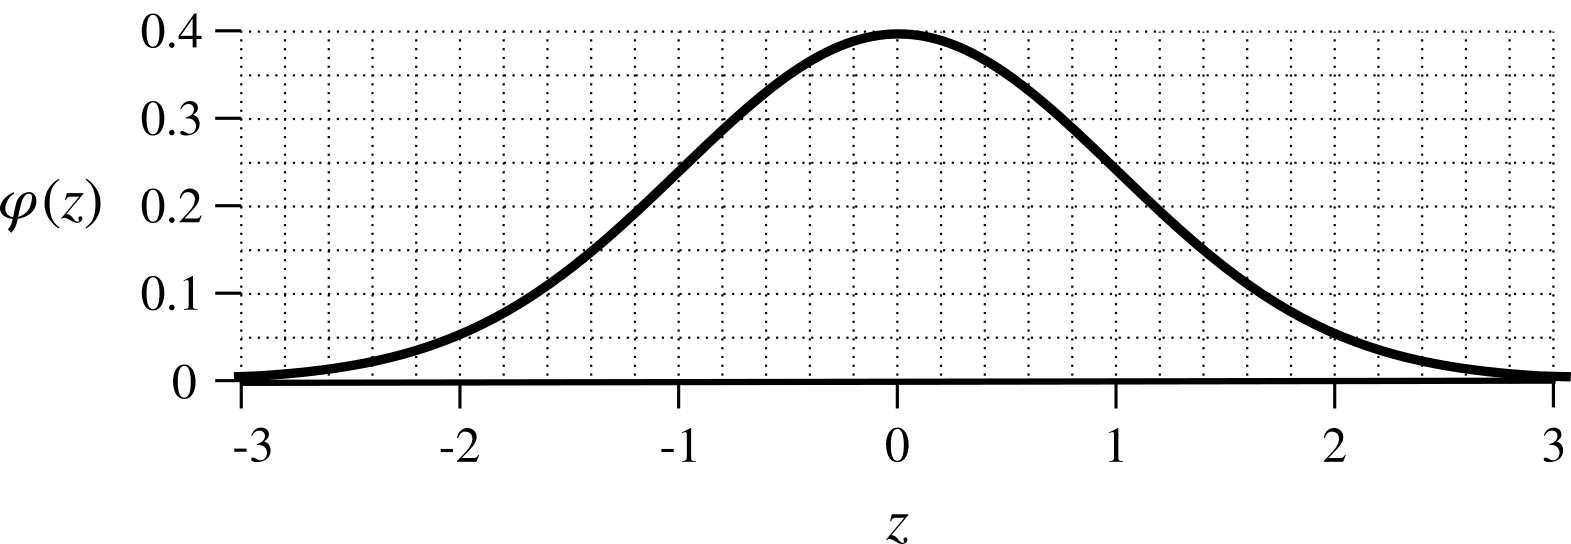
\includegraphics[scale=0.7]{blank.png}   $~~\emptybox=\emptybox$
\vfill
\item Shade the region of and evaluate the probability that $Z$ is between -0.4 and 0.4.
\\ 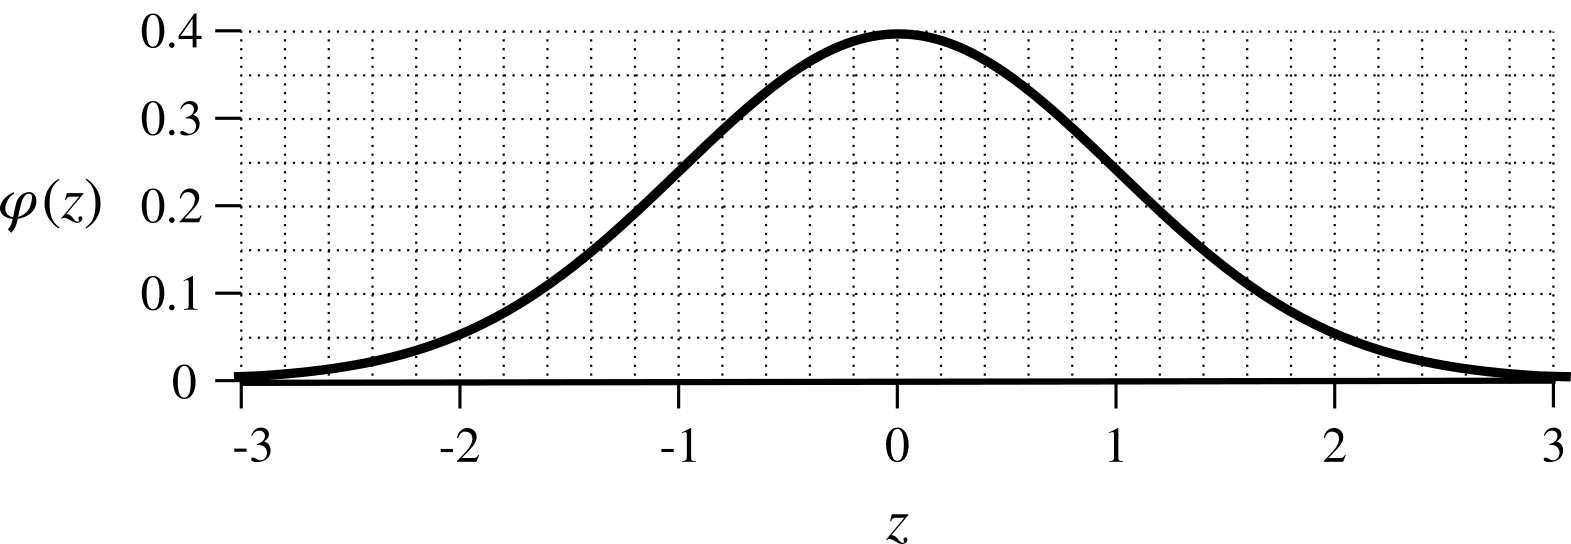
\includegraphics[scale=0.7]{blank.png}   $~~\emptybox=\emptybox$
\vfill
\item Shade the region of and evaluate the probability that $Z$ is less than -0.4 or more than 0.4.
\\ 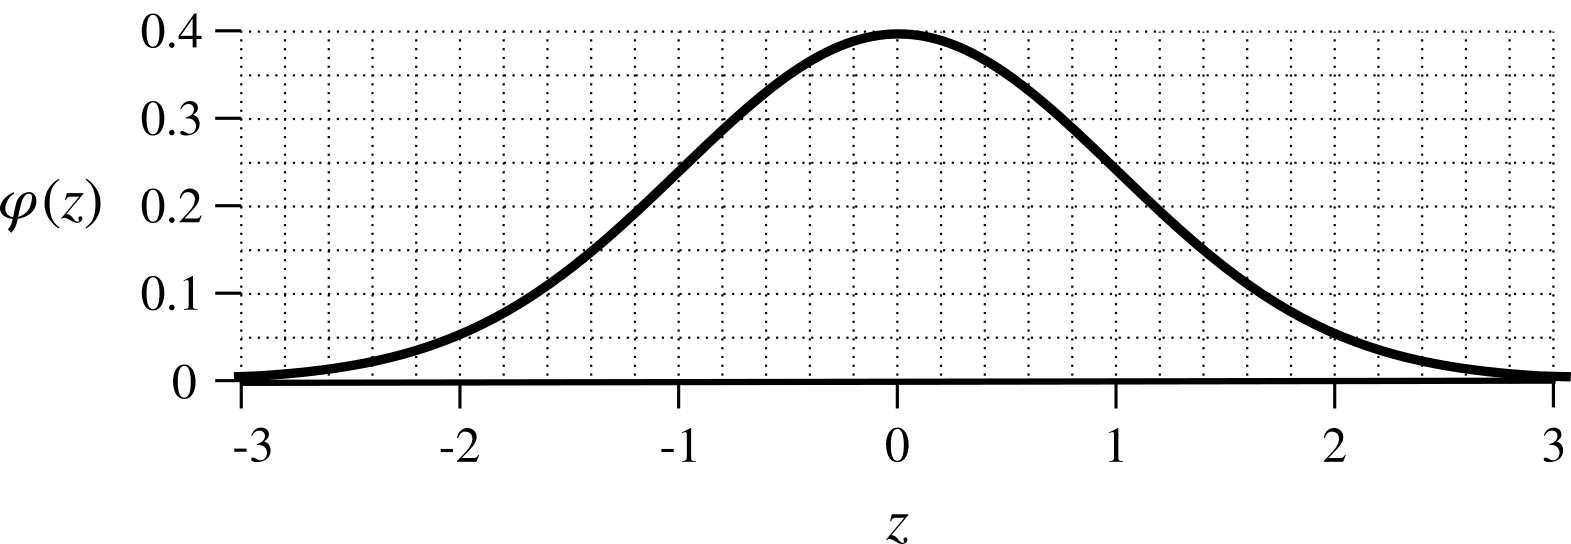
\includegraphics[scale=0.7]{blank.png}   $~~\emptybox=\emptybox$
\vfill
\end{enumerate}
\end{enumerate}



%\newpage
%\begin{enumerate}
%\item Evaluate $\Phi(1.96)$
%\vfill
%\item Evaluate $P(Z < 1.08)$
%\vfill
%\item Evaluate $P(Z > 1.08)$
%\vfill
%\item Evaluate $P(1.08 < Z < 1.96)$
%\vfill
%\item Evaluate $P(|Z| < 1.96)$, which is the same as $P(-1.96 < Z < 1.96)$
%\vfill
%\item Evaluate $P(|Z| > 1.96)$, which is the same as $P(Z < -1.96 ~~\text{OR}~~ 1.96<Z)$
%\vfill
%\end{enumerate}


\newpage
This diagram might be useful. Some of the areas seem to add imperfectly because these numbers are all rounded. Also, it should be noted that $\Phi(-3) = 0.00135 \ne 0$.\\\\
\begin{center}
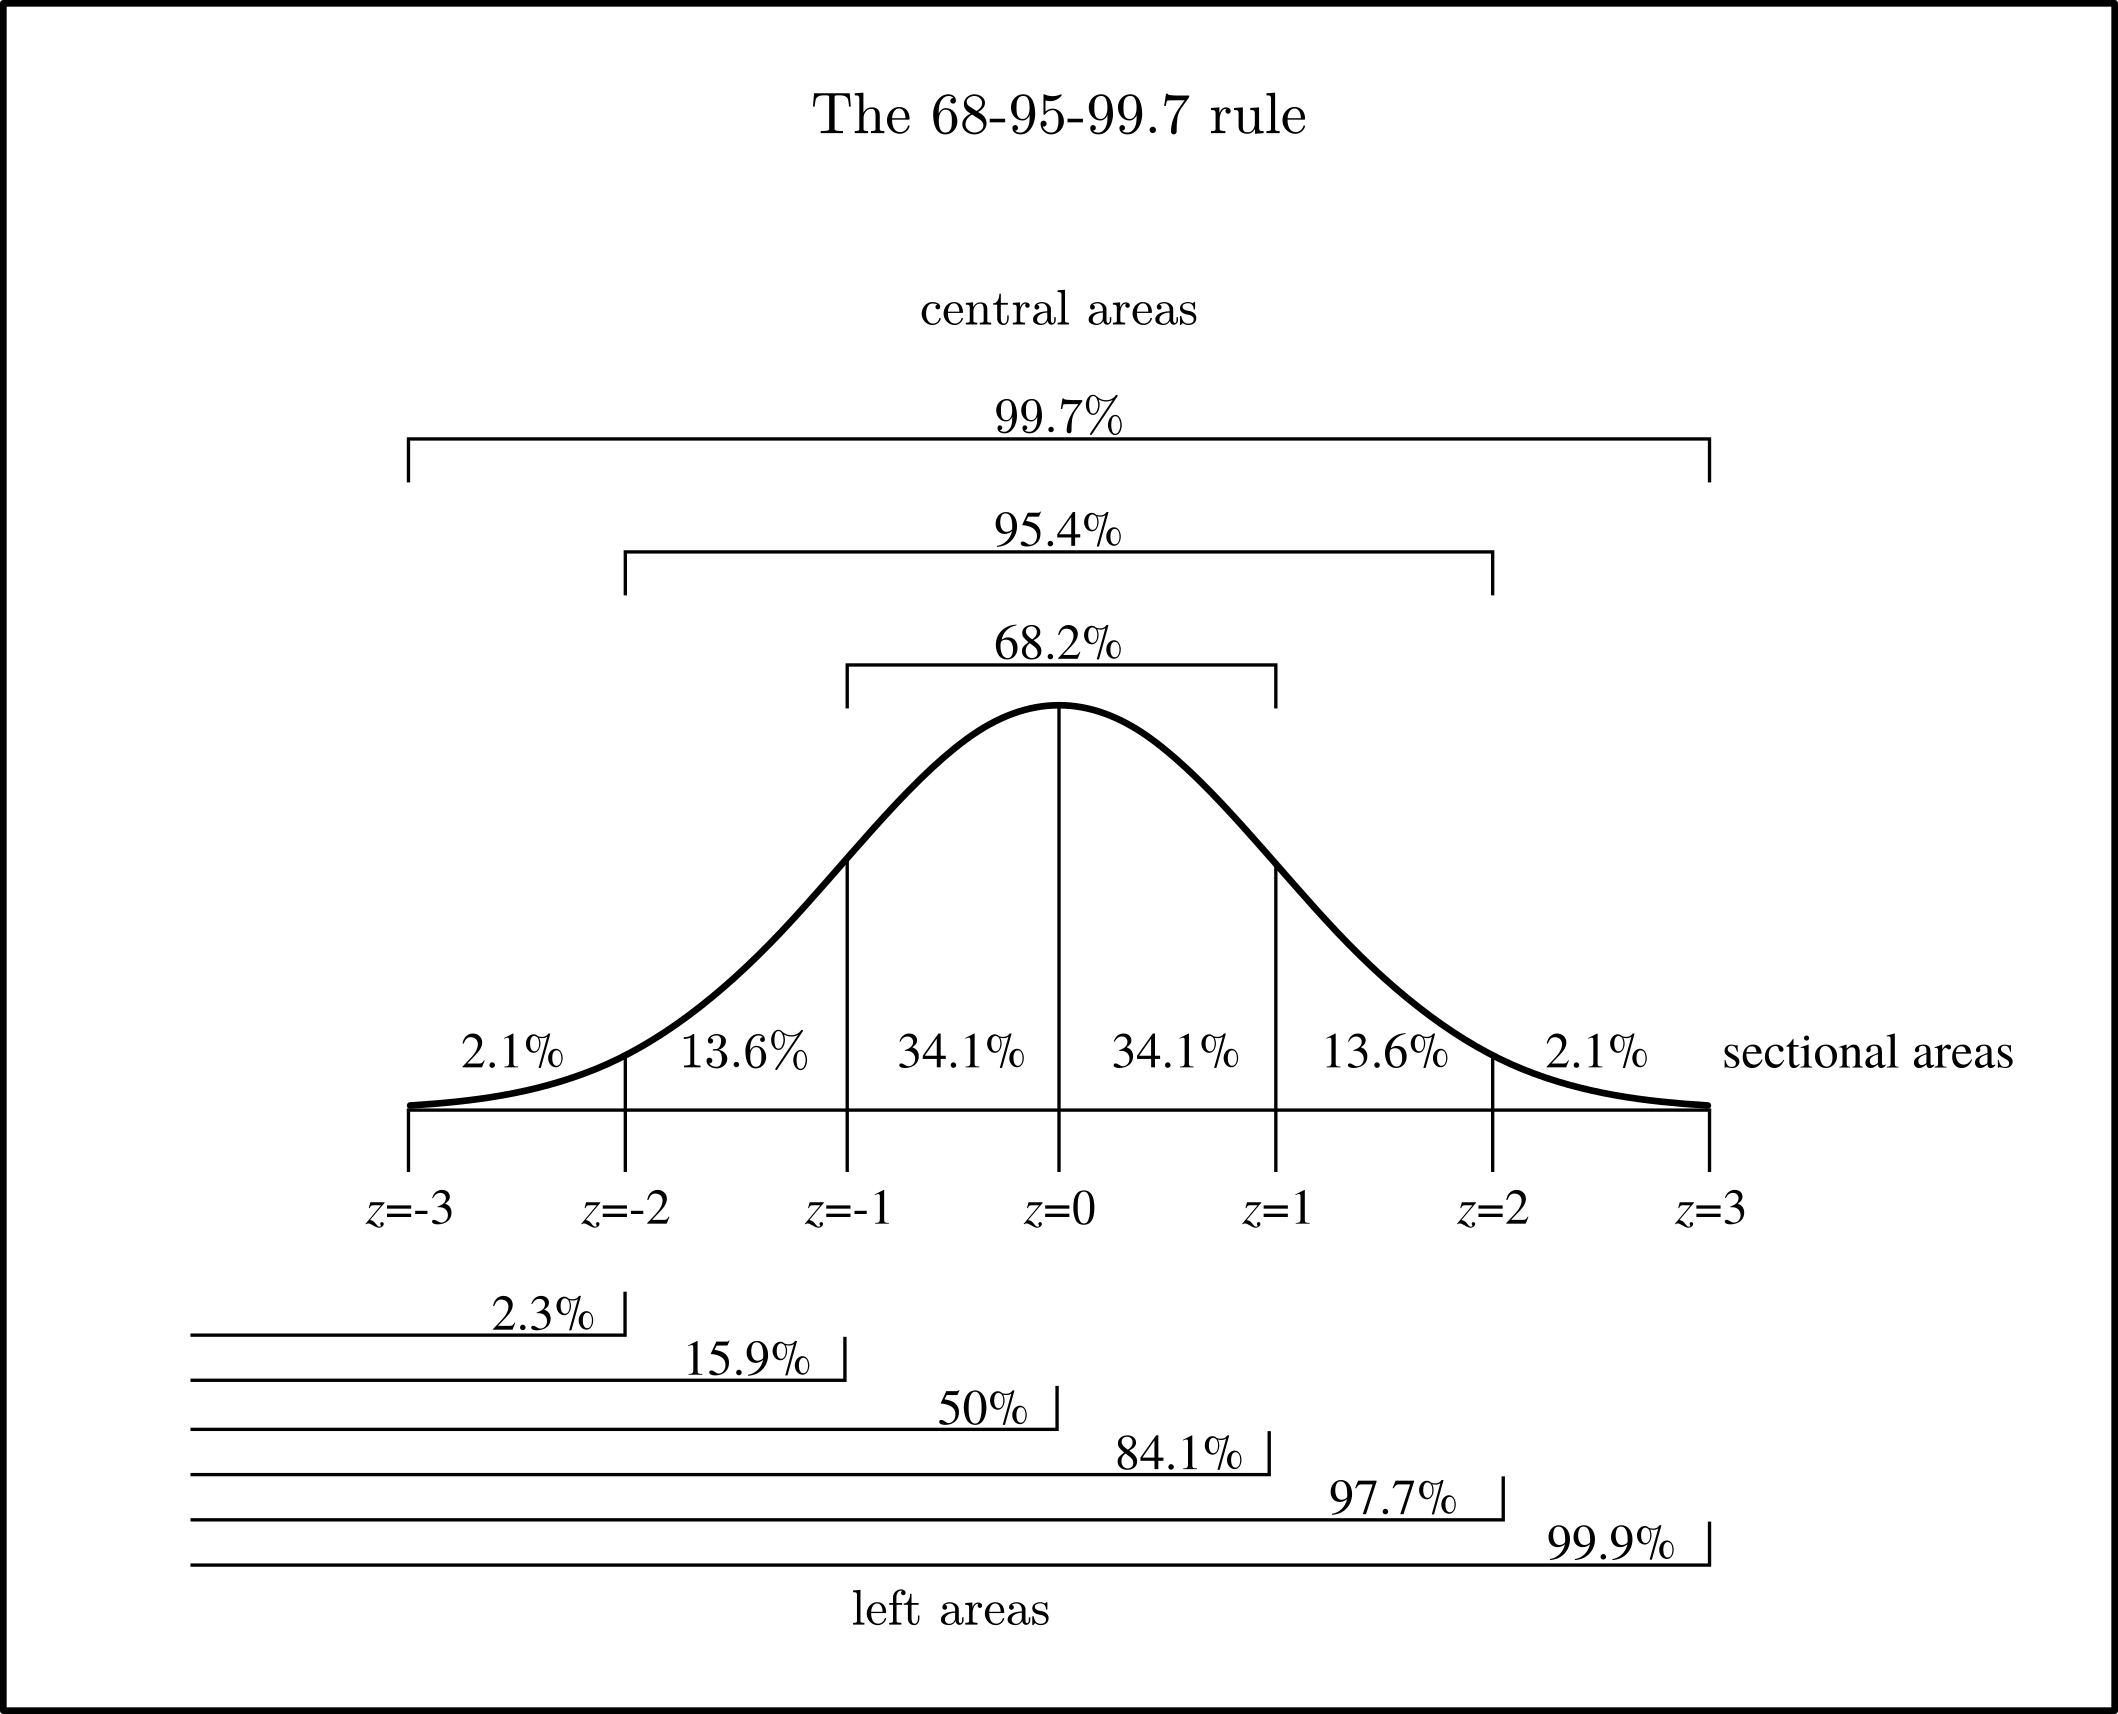
\includegraphics[scale=1]{toomuch.png}
\end{center}
\url{https://en.wikipedia.org/wiki/68-95-99.7_rule}




\newpage
\begin{enumerate}[resume]
\item By using the standard normal table (or the 68-95-99.7 rule), you should be able to determine the following probabilities. For each question, determine the probability (area) of the shaded region or regions. In cases where the bound could be $-3$ or $3$, use $-\infty$ or $\infty$ instead.  Write the answer using the ``$P(\texttt{condition}) = \texttt{number}$'' format.

\begin{enumerate}[itemsep=50pt]
\begin{multicols}{2}
\item \adjustbox{valign=t}{
\includegraphics[scale=.5]{n3_n1.png}}
\item \adjustbox{valign=t}{
\includegraphics[scale=.5]{n3_0.png}}
\item \adjustbox{valign=t}{
\includegraphics[scale=.5]{n3_1.png}}
\item \adjustbox{valign=t}{
\includegraphics[scale=.5]{n1_3.png}}
\item \adjustbox{valign=t}{
\includegraphics[scale=.5]{0_1.png}}

\columnbreak

\item \adjustbox{valign=t}{
\includegraphics[scale=.5]{0_2.png}}
\item \adjustbox{valign=t}{
\includegraphics[scale=.5]{n1_1.png}}
\item \adjustbox{valign=t}{
\includegraphics[scale=.5]{n2_2.png}}
\item \adjustbox{valign=t}{
\includegraphics[scale=.5]{n3_n2_and_2_3.png}}
\item \adjustbox{valign=t}{
\includegraphics[scale=.5]{n3_n1_and_1_3.png}}

\end{multicols}
\end{enumerate}
\end{enumerate}

\newpage
\noindent We have practiced finding areas from $z$-scores. We might also want to find $z$-scores from areas. You'll need to use your standard normal table backwards.
\begin{enumerate}[resume]
\item \begin{enumerate}
\item Determine $z_0$ such that $\Phi(z_0)=0.0505$.
\vfill
\item Determine $z_1$ such that $\Phi(z_1)\approx 0.99$.
\vfill
\item Determine $z_2$ such that $P(Z < z_2) = 55.57\%$
\vfill
\item Determine $z_3$ such that $P(Z > z_3) = 15.87\%$
\vfill
\item Determine $z_4$ such that $P(-z_4 < Z < z_4) = 68.2\%$
\vfill
\item Determine $z_5$ such that $P(|Z| < z_5) = 95\%$
\vfill
\item Determine $z_6$ such that $P(|Z| < z_6) = 90\%$
\vfill
\item Determine $z_7$ such that $P(|Z| > z_7) = 10\%$
\vfill
\end{enumerate}

\newpage
\item If the scores on a test are normally distributed with a mean of 80 and a standard deviation of 10, what score is the 84.1th percentile? (Hint: check out the 68-95-99.7 rule.)
\vfill
\item If the scores on a test are normally distributed with a mean of 80 and a standard deviation of 10, what score is the 97.7th percentile?
\vfill
\item If the scores on a test are normally distributed with a mean of 80 and a standard deviation of 10, what score is the 90th percentile?
\vfill
\item What is the $z$-score such that 68.2\% of the area lies between $-z$ and $z$? (Hint: check out the 68-95-99.7 rule.)
\vfill
\item What is the $z$-score such that 95.4\% of the area lies between $-z$ and $z$?
\vfill
\item What is the $z$-score such that 80\% of the area lies between $-z$ and $z$?
\vfill


\end{enumerate}
\newpage
	\setenumerate[1]{label={\bf A\theenumi: ~}}
	\setenumerate[2]{label={\bf \theenumii: ~}}
\begin{multicols}{2}
\begin{enumerate}
\item \begin{enumerate}
\item $P\bigl(Z < -1.4\bigr) = 0.0808 $\\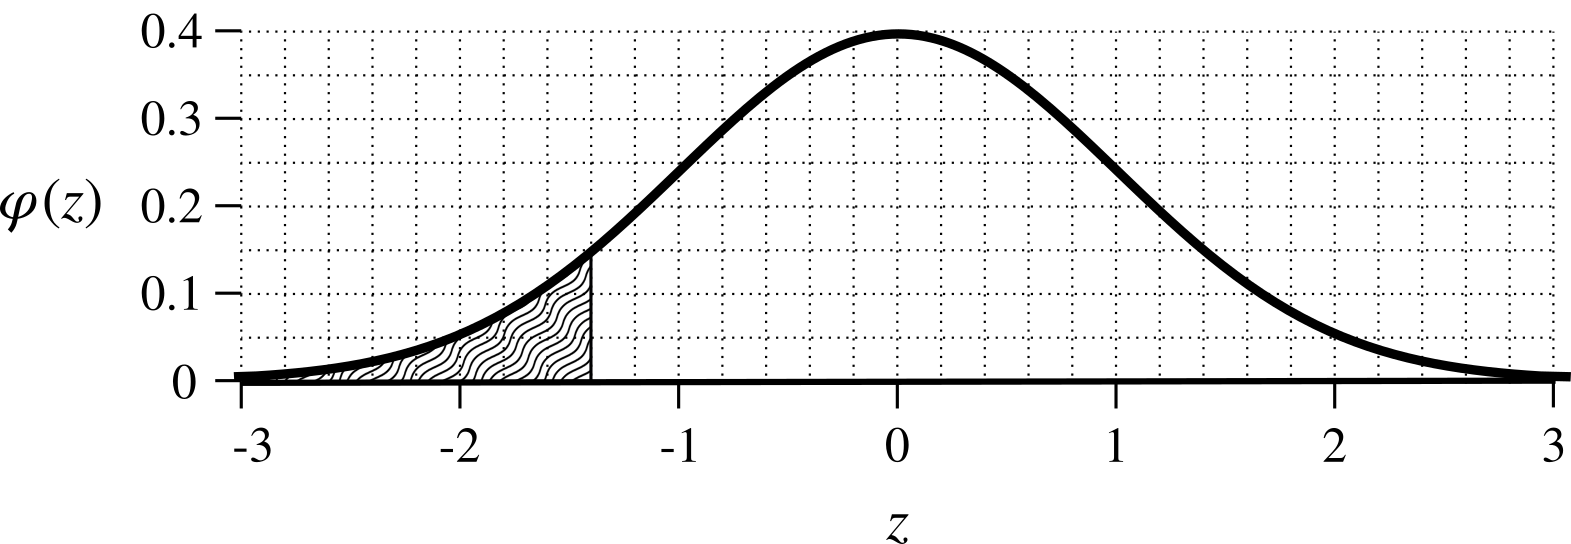
\includegraphics[scale=0.4]{n1p4.png}
\item $P\bigl(Z < 2\bigr) = 0.9772 $\\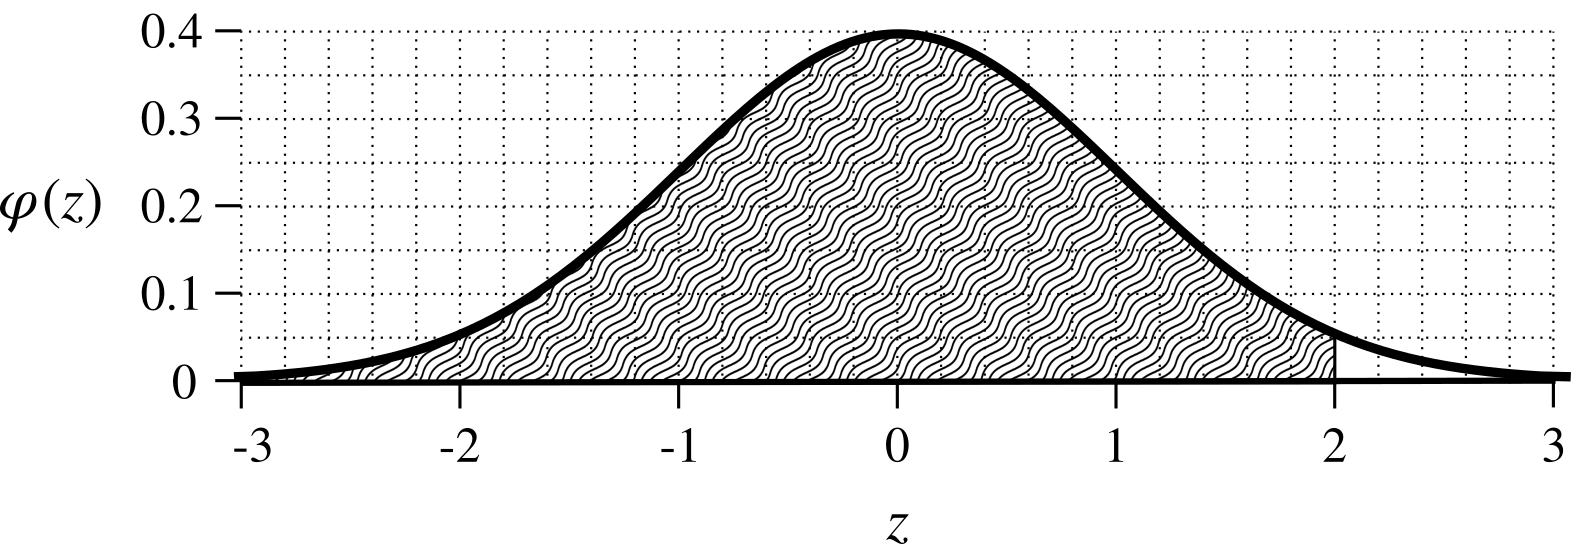
\includegraphics[scale=0.4]{2.png}
\item $P(Z<-0.2) = 0.4207$
\end{enumerate}

\item \begin{enumerate}
\item $P\bigl(Z > 1.6\bigr) = 0.0548 $\\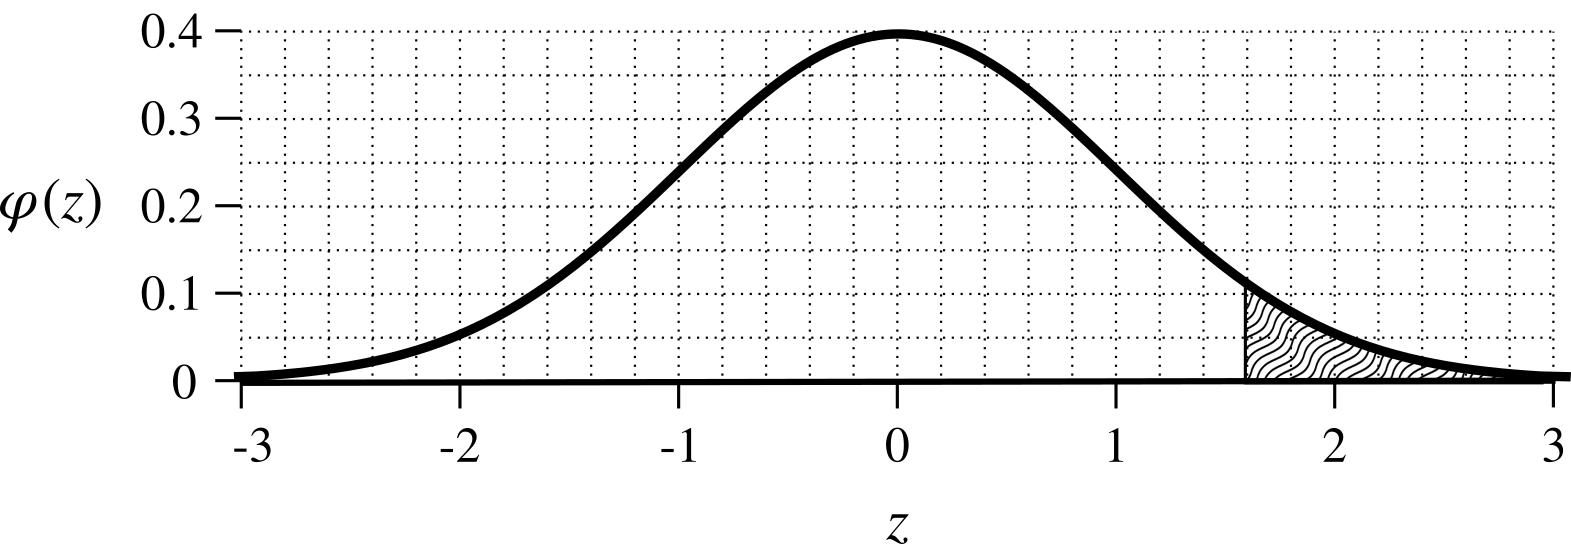
\includegraphics[scale=0.4]{g1p6.png}
\item $P\bigl(0.4 < Z < 0.6\bigr) = 0.0703 $\\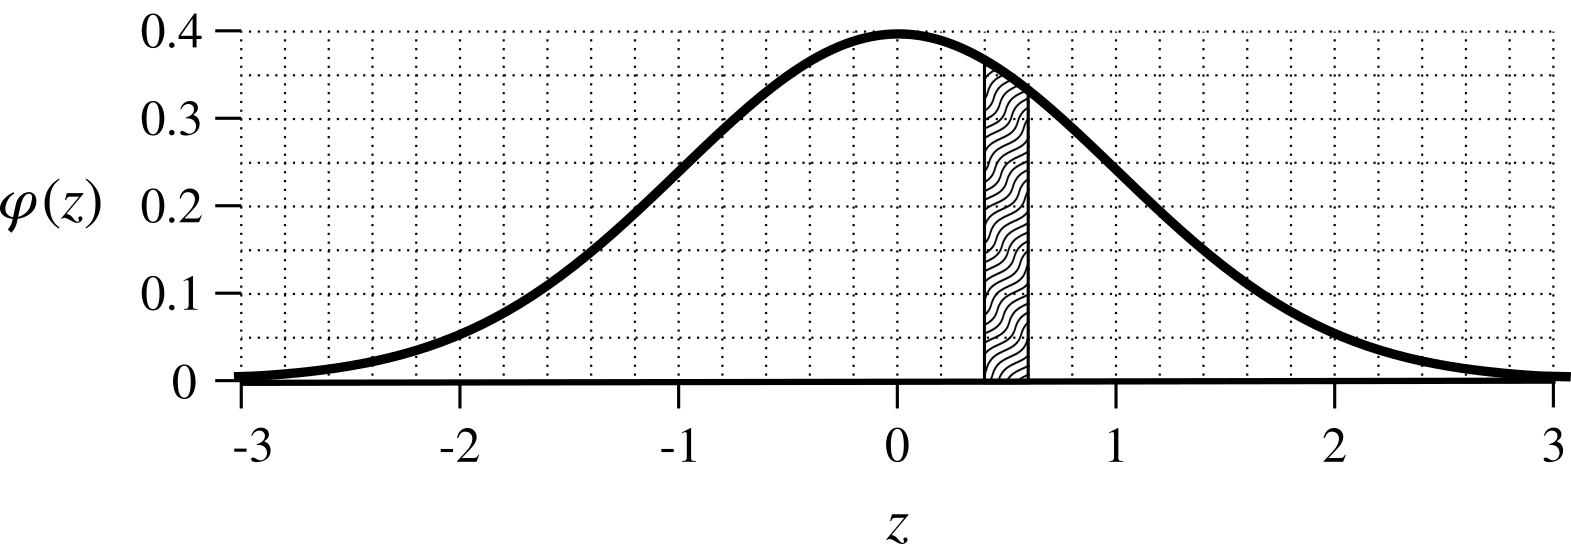
\includegraphics[scale=0.4]{bp4p6.png}
\item $P\bigl(1 < Z < 2\bigr) = 0.1359 $\\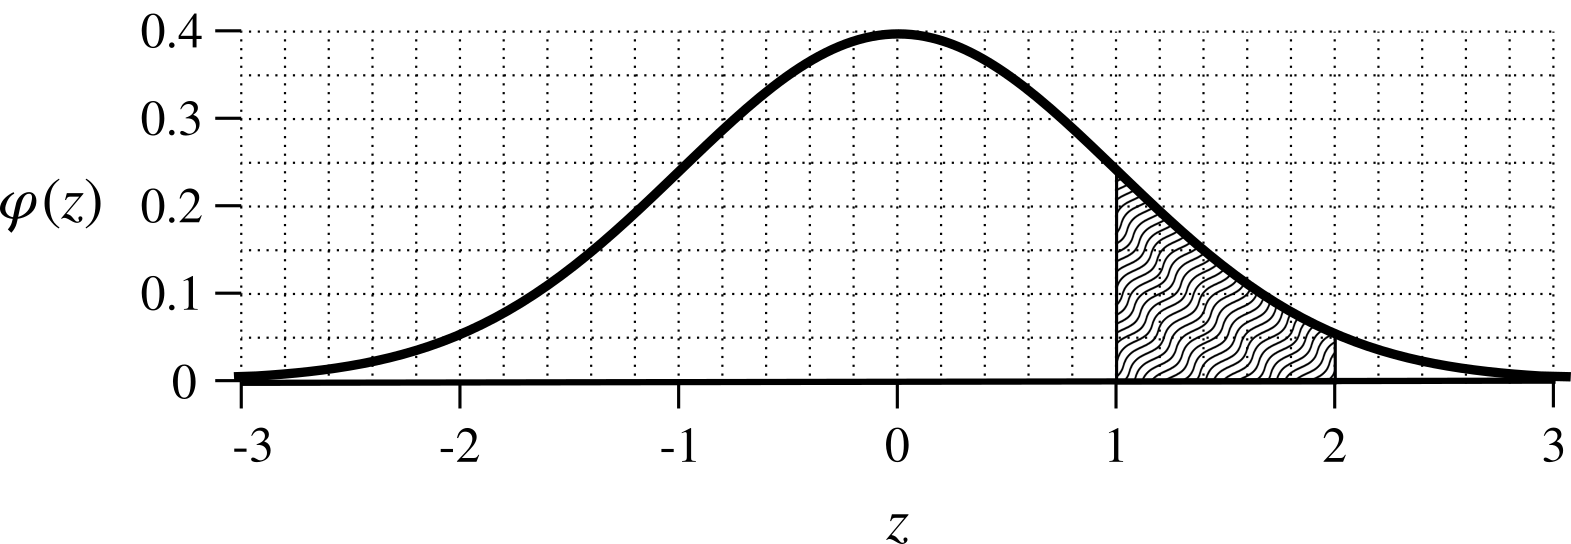
\includegraphics[scale=0.4]{b1a2.png}
\item $P\bigl(|Z| < 0.4\bigr) = 0.3108 $\\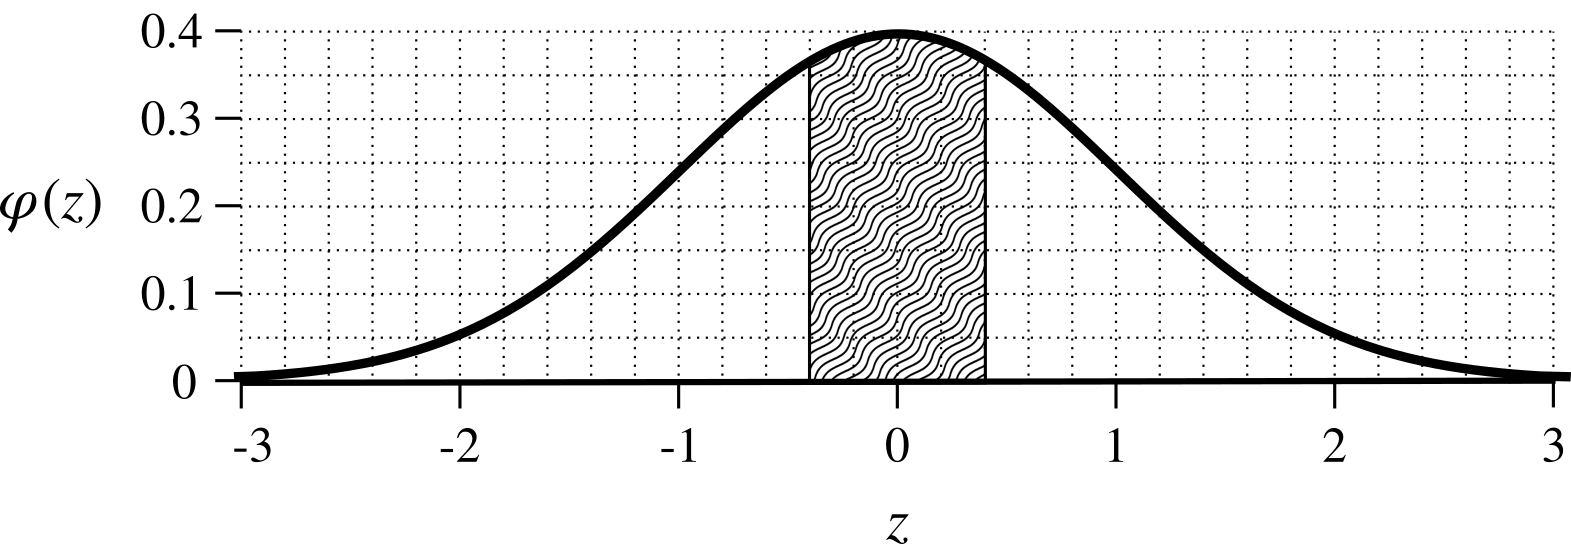
\includegraphics[scale=0.4]{alp4.png}
\item $P\bigl(|Z| > 0.4\bigr) = 0.6892 $\\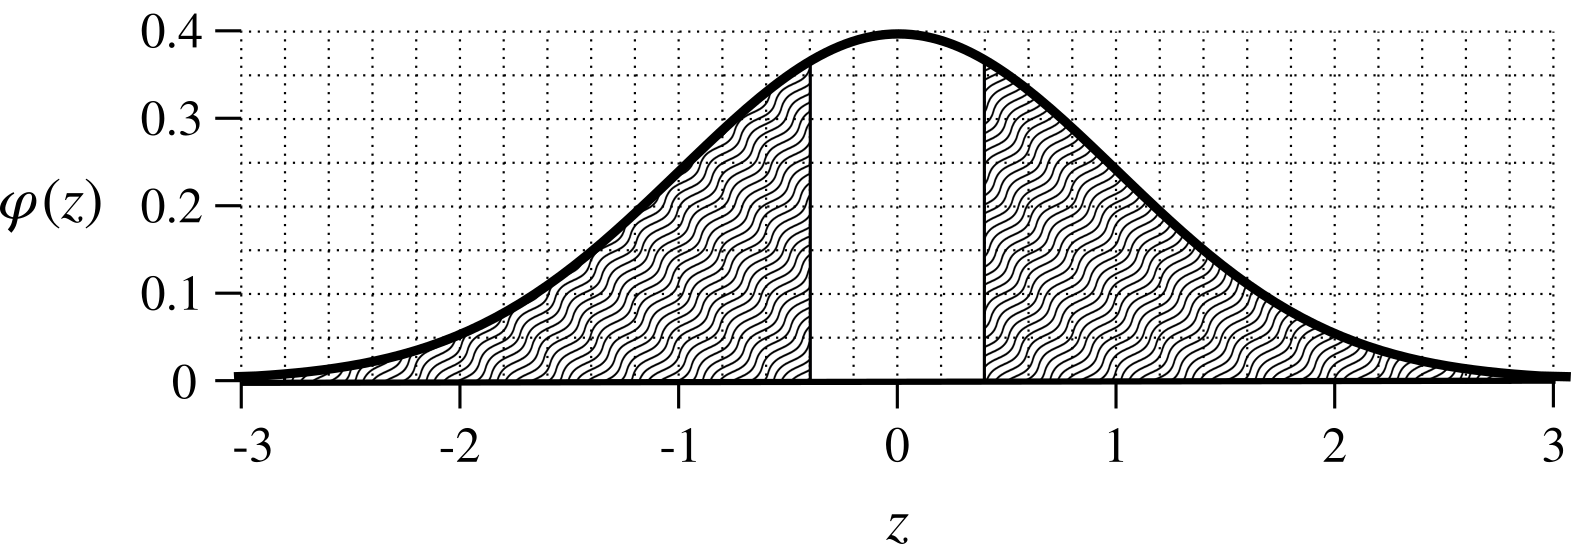
\includegraphics[scale=0.4]{agp4.png}
\end{enumerate}
\columnbreak
\item \begin{enumerate}
\item $P(Z<-1)=0.159$
\item $P(Z<0) = 0.5$
\item $P(Z<1) = 0.841$
\item $P(-1<Z) = 0.841$
\item $P(0<Z<1) = 0.341$
\item $P(0<Z<2) = 0.477$
\item $P(|Z|<1) = 0.682$
\item $P(|Z|<2) = 0.954$
\item $P(|Z|>2) = 0.046$
\item $P(|Z|>1) = 0.318$
\end{enumerate}


\item \begin{enumerate}
\item $z_0 = -1.64$
\item $z_1 = 2.33$
\item $z_2 = 0.14$
\item $z_3 = 1$
\item $z_4 = 1$
\item $z_5 = 1.96$
\item $z_6 = 1.64$
\item $z_7 = 1.64$
\end{enumerate}

\item 90.0
\item 100.0
\item $z = 1.28
\\(1.28)(10)+80 \approx \fbox{92.8}$
\item $z=1$
\item $z=2$
\item $z =1.28$

\end{enumerate}
\end{multicols}

\end{document}
